\documentclass{sig-alternate}

\hyphenation{data-bases}

\newcommand{\TITLE}{Peer comparison of XSEDE and NCAR publication data}
\newcommand{\AUTHOR}{Gregor von Laszewski, Fugang Wang}

%%%%%%%%%%%%%%%%%%%%%%%%%%%%%%%%%%%%%%%%%%%%%%%%%%%%%%%%%%%%%%
% LATEX DEFINITIONS 
%%%%%%%%%%%%%%%%%%%%%%%%%%%%%%%%%%%%%%%%%%%%%%%%%%%%%%%%%%%%%%

\usepackage{float}
\usepackage{comment}
\usepackage{hyperref} 
\usepackage{array} 
\usepackage{graphicx} 
\usepackage{booktabs} 
\usepackage{pifont} 
\usepackage{todonotes} 
\usepackage{rotating} 
\usepackage{color} 
\usepackage{caption}
\captionsetup{font={scriptsize}}

\newcommand*\rot{\rotatebox{90}} 
 
\newcommand{\FILE}[1]{\todo[color=green!40]{#1}} 
 

%
% more floats on one page
%
\renewcommand{\topfraction}{.85}
\renewcommand{\bottomfraction}{.7}
\renewcommand{\textfraction}{.15}
\renewcommand{\floatpagefraction}{.66}
\renewcommand{\dbltopfraction}{.66}
\renewcommand{\dblfloatpagefraction}{.66}
\setcounter{topnumber}{9}
\setcounter{bottomnumber}{9}
\setcounter{totalnumber}{20}
\setcounter{dbltopnumber}{9}

%%%%%%%%%%%%%%%%%%%%%%%%%%%%%%%%%%%%%%%%%%%%%%%%%%%%%%%%%%%%%%
% HYPERSETUP 
%%%%%%%%%%%%%%%%%%%%%%%%%%%%%%%%%%%%%%%%%%%%%%%%%%%%%%%%%%%%%%

\hypersetup{ 
    bookmarks=true,         % show bookmarks bar 
    unicode=false,          % non-Latin characters in Acrobat's bookmarks 
    pdftoolbar=true,        % show Acrobat's toolbar 
    pdfmenubar=true,        % show Acrobat's menu 
    pdffitwindow=false,     % window fit to page when opened 
    pdfstartview={FitH},    % fits the width of the page to the window 
    pdftitle={\TITLE},    % title 
    pdfauthor={\AUTHOR},     % author 
    pdfsubject={Subject},   % subject of the document 
    pdfcreator={Gregor von Laszewski, Fugang Wang},   % creator of the document 
    pdfproducer={}, % producer of the document 
    pdfkeywords={hindex} {metric}{XSEDE} {FutureGrid}, % list of keywords 
    pdfnewwindow=true,      % links in new window 
    colorlinks=false,       % false: boxed links; true: colored links 
    linkcolor=red,          % color of internal links (change box color with linkbordercolor) 
    citecolor=green,        % color of links to bibliography 
    filecolor=magenta,      % color of file links 
    urlcolor=cyan           % color of external links 
} 

\begin{document}


%\conferenceinfo{submitted to XSEDE}{'15,  July 26 - 30 2015, St. Louis, MO, USA}
\conferenceinfo{submitted to ...}{2015,USA}
\CopyrightYear{2015} 
\crdata{TBD...\$15.00.\\
http://dx.doi.org/TBD
} 


\title{\TITLE\vspace{-12pt}}


\numberofauthors{3}  
\author{ 
\alignauthor 
Gregor von Laszewski\titlenote{Corresponding Author.}\\ \vspace{2pt}
Fugang Wang\\ \vspace{2pt}
Geoffrey C. Fox\\ \vspace{6pt}
       \affaddr{Indiana University}\\ 
       \affaddr{2719 10th Street}\\ 
       \affaddr{Bloomington, Indiana, U.S.A.}\\ 
\and  
\alignauthor  David L. Hart\\ \vspace{6pt}
       \affaddr{Computational and Information Systems Laboratory National Center for Atmospheric Research}\\
       \affaddr{P.O. Box 3000}\\
       \affaddr{Boulder CO 80307-3000}\\
\and
\alignauthor  
Thomas R. Furlani\\ \vspace{2pt}
Robert L. DeLeon\\ \vspace{2pt}
Steven M. Gallo\\ \vspace{6pt}
       \affaddr{Center for Computational Research}\\
       \affaddr{University at Buffalo, SUNY}\\ 
       \affaddr{701 Ellicott Street}\\ 
       \affaddr{Buffalo, New York, 14203}
}

\date{28 May 2014}

\maketitle

\begin{abstract}

We present a framework that compares the publication impact based on a comprehensive peer analysis of papers produced by scientists using XSEDE and NCAR resources. The analysis is introducing a percentile ranking of citations of the XSEDE and NCAR papers compared to peer publications in the same journal that do not use these resources.  This analysis is unique in that it is a comprehensive study in which all reported published papers are compered to peer publications selected from within the same issue of the same journal. From this analysis, we can see that papers that utilize XSEDE and NCAR resources are cited statistically significantly more often.  Hence we find that reported publications indicate that XSEDE and NCAR resources exert a strong positive impact on scientific research.

\end{abstract}


\vspace{-6pt}

\category{H.4}{Information Systems Applications}{Miscellaneous}
\category{D.2.8}{Software Engineering}{Metrics}[complexity measures,
performance measures]

\terms{Theory, Measurement}

\keywords{Scientific impact, bibliometric, h-index, Technology Audit
  Service, XDMoD, XSEDE}


\section{Introduction} 

To identify the impact on {\em scientific advancements enabled by enhanced cyberinfrastructure}, it is important to conduct a comprehensive analysis of achievements that can be attributed to the use of advanced infrastructure, such as provided by the Extreme Science and Discovery Environment (XSEDE) \cite{www-xsede,xsede}. Many recent science and engineering innovations and discoveries are increasingly dependent on access to high-end computing resources \cite{las14impact}. The demand for high-end resources is met by large-scale compute resources located in geographically dispersed locations that cannot typically be supported by any single research group. Accordingly, dedicated large-scale computing facilities play an important role in scientific research, in which resources are shared among groups of researchers, while the facilities themselves are managed by dedicated staff. The National Science Foundation (NSF) and the Department of Energy have supported such facilities for many years. XSEDE allocates resources to approved projects, which represent a substantial financial investment by NSF. Thus, justification for their use is warranted and questions regarding the scientific impact of these resources naturally arise. In previous work \cite{las14impact} we focused on the creation of a framework that collects bibliometric data and analyzes them with respect to a number of metrics. However, this work did not yet include a mechanism to compare publications with peers not using such resources.

In this paper, we significantly enhance our previous work by comparing publication impact based on a comprehensive peer analysis carried out on papers produced by scientists using XSEDE and National Center for Atmospheric Research (NCAR) resources. The analysis is based on a percentile ranking of citations of the papers derived from a comparison to peer publications in the same journal not using the resources.  This analysis is unique in that it is a comprehensive study in which thousands of published papers are are compered to peer publications selected from within the same issue of the same journal. From this analysis we can see that papers that utilize XSEDE and NCAR resources are cited statistically significantly more often.  

The paper is structured as follows. First, we review some portions of our previous work and relate it to the work reported in this paper (Section~\ref{S:related}). We review our design and the architecture of our framework supporting this effort (Section~\ref{S:framework}). Next we introduce a journal-based peer metric that allows us to compare any resource provider's related publications with publications not using the resources (Section~\ref{S:metric}).  To demonstrate general applicability of this method, we introduce in the next section a peer analysis of XSEDE (Section \ref{S:xsede}) and NCAR data (Section~\ref{S:ncar}). We present important statistics about this metric for both XSEDE and NCAR. Finally, we present our conclusions (Section~\ref{S:conclusion}).

\section{Related Work} \label{S:related}

Although a number of related studies have been conducted
\cite{thomas1998institutional,
  Bollen:2007:MUM:1255175.1255273,Bollen:2008:TUI:1378889.1378928,
  bollen2009principal,bollen2011and} our work is unique in that it provides a {\em comprehensive} analysis superior in data volume to other studies and is focused on the analysis of XSEDE and NCAR data. More information about related work can be found in \cite{las14impact}. We are happy to engage in collaborative efforts to enhance this work or to integrate other related work by contacting us.

\section{Bibliometric Data Analysis \\Framework for Resource
  \\Providers} \label{S:framework}

The work described in this paper has been motivated by analyzing data related to XSEDE\footnote{The XSEDE data set includes publications from both XSEDE and its predecessor program, TeraGrid. For simplicity, we refer to {\em XSEDE} throughout this paper.}. However, as many other resource providers may have similar needs to analyze their data, this framework is general enough that it can be adapted for use by other resource providers. In case this is desired, a custom integration can be performed and the analysis can be adapted by the team from Indiana University. 


\subsection{Requirements}

The motivation for the framework includes three main objectives.  First, our framework must be able to compare the impact of the use of resources on their users. Second, we have to define suitable metrics that allow such a comparison. Third, we need to provide a framework that provides an integrated set of data services on which these metrics can be applied to conduct a comparative impact analysis. This is depicted in Figure \ref{F:objectives} on the left-hand side.

\subsection{Design}

% NOTE: OTHERS DELETED

For XSEDE we have identified specific design criteria that we are integrating into our architecture. Many of these design decisions will overlap with other resource providers. Certainly our design needs to be able to provide a comparative impact study for peers and also the funding agencies of the peers in conjunction with meaningful metrics. The metrics must be not only targeting the resource provider but also the community. Specifically for XSEDE interested parties in this analysis are not only the users, but also the Resource Allocation Committee (RAC) and the XSEDE leadership. The bibliometric data services and the data mashup are largely hidden from these groups. The groups benefit form a number of preconfigured analysis that may be further customized or enhanced. To show generality of this approach we have taken an analysis and applied it not only to XSEDE as a resource provider, but also to National Center for Atmospheric Research (NCAR) as a resource provider \cite{www-ncar}.

\begin{figure}[htb] 
  \centering 
    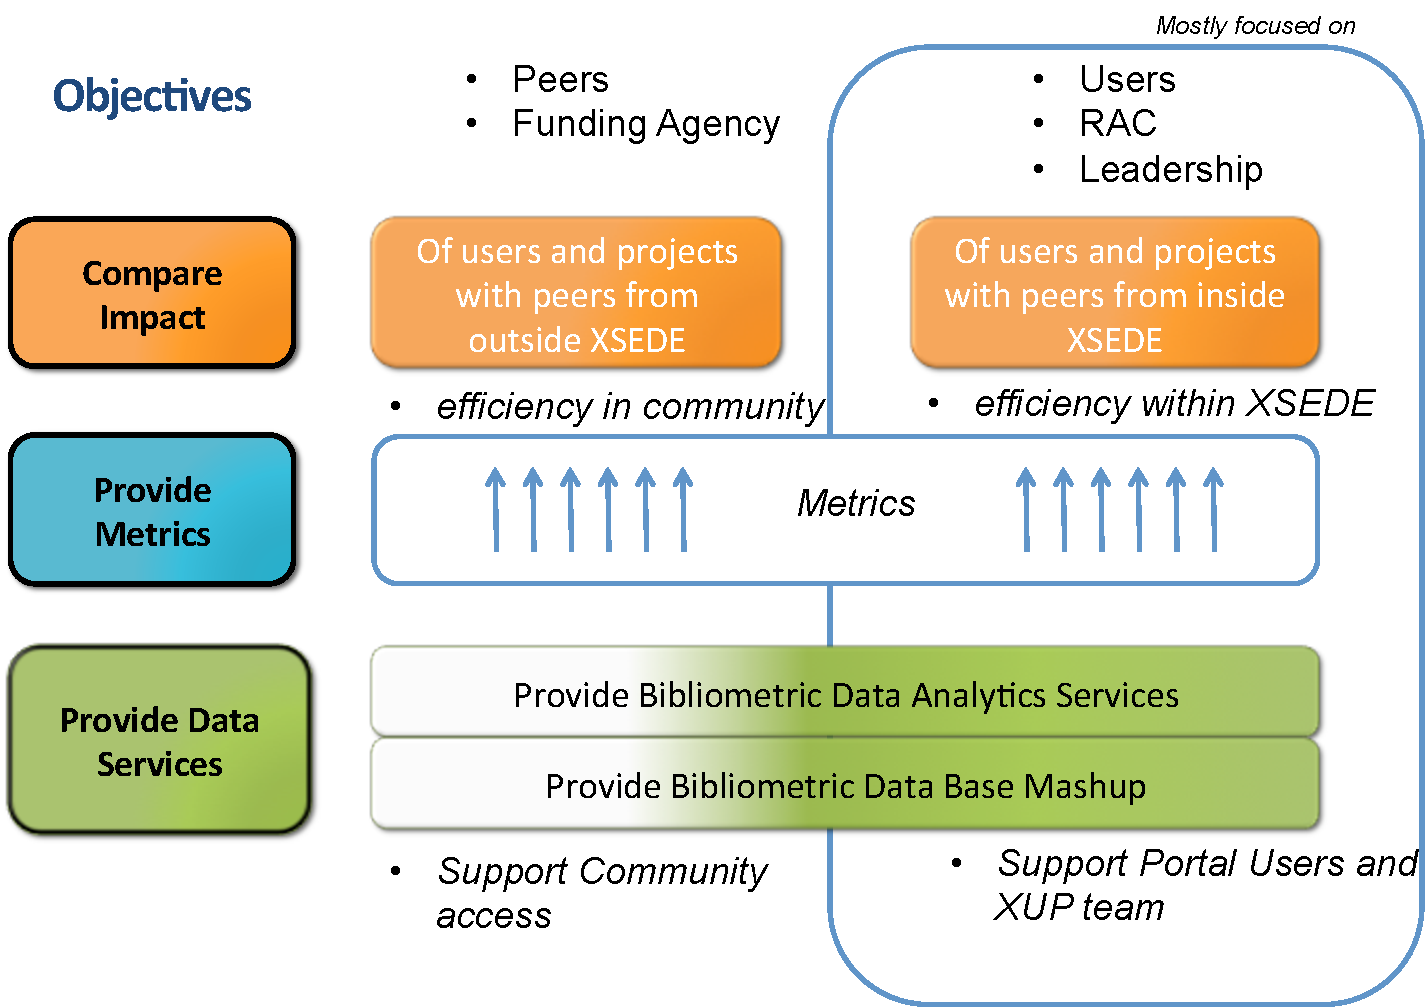
\includegraphics[width=1.0\columnwidth]{images-new/objectives.pdf} 
    \caption{High level Objectives impacting the design of our framework}
    \label{F:objectives}
\end{figure} 

\begin{figure}[htb] 
  \centering 
    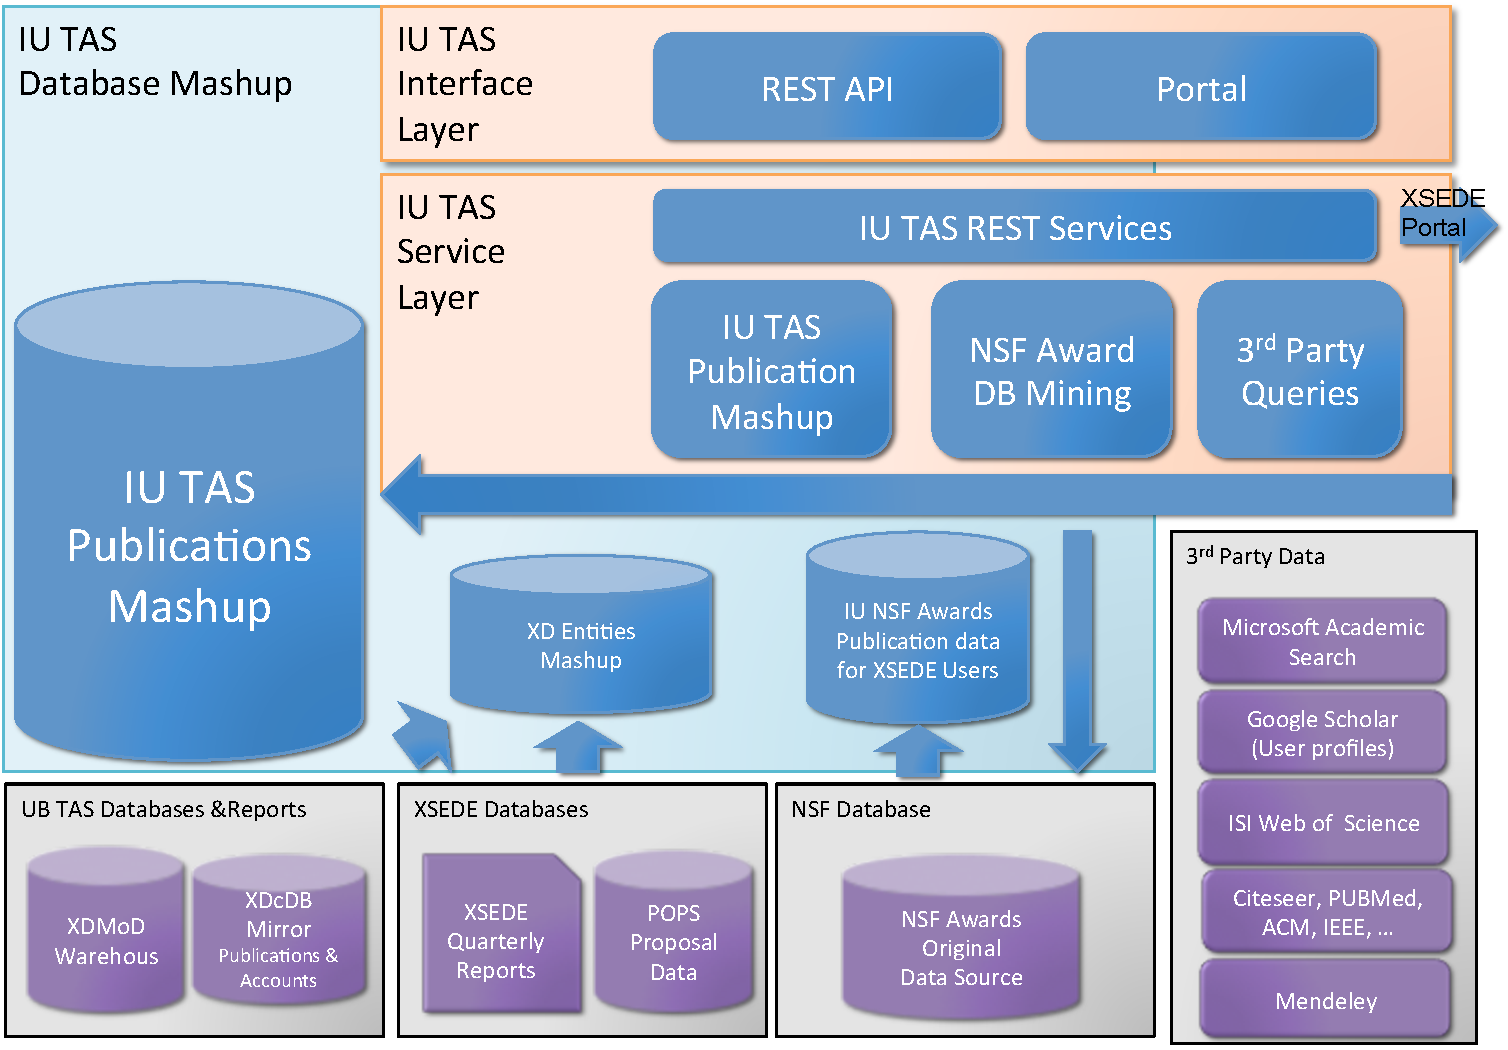
\includegraphics[width=1.0\columnwidth]{images-new/architecture.pdf} 
  \caption{Architecture with the Interface, Service, Database Mashup,
    and Database Resources Layers}\label{F:architecture} 
\end{figure} 

\subsection{Architecture}

%\footnote{produced using XSEDE resources}
The requirements for XSEDE and our user community have resulted in a layered architecture as depicted in \ref{F:architecture}.  The framework is based on a distributed set of services.  The service-oriented system consists of components for (a) publication and citation data retrieval (e.g., from the NSF award database, Google Scholar, and ISI Web of Science); (b) parsing and processing while correlating data from various databases and services, such as the XSEDE central database (XDCDB), which stores all usage data for jobs run on XSEDE resources; and (c) the XSEDE allocations database, which stores publication and grant funding information for PIs applying for XSEDE allocations.  The system also includes components for metrics generation and an analysis system for different aggregation levels -- users, projects, organization, field of science (FOS) -- as well as a presentation layer using a lightweight portal in addition to exposing some data via a RESTful API \cite{las14impact}.  The main layers include (a) {\em Interface Layer} -- easy to use interfaces for various communities, including an API, REST, and a Web GUI interface; (b) {\em Service Layer} -- advanced services to bridge to a database mashup via sophisticated services and queries to the underlying database layer; (c) {\em Database Mashup Service Layer} -- a sophisticated database mashup that contains the integration of data from a variety of data resources; and (d) the {\em Database Resources} that provide the underlying information for our service.

Due to this approach, our framework is expandable as we are able to integrate not only resources relevant for XSEDE, but also other resource providers such as NCAR. However, we need to customize this integration and allow relevant services to be exposed to the framework. In some cases it could be as simple as replacing the database with a minor adaptation in the service layer.



Our current framework for XSEDE includes specialized services focusing on XSEDE user specific publication data as well as user, project, and FOS views. The mashup component aggregates the publication data mined from the previous component, in addition to those from XDCDB, and from other available external services. It also retrieves citation data for each publication from external services. Another essential task of this framework is to generate metrics for users, projects, and FOS, in which the XSEDE allocations database is involved to get proposal and project data. These data will be stored in the mashup database, which can then be integrated into the XDMoD system \cite{Furlani:2013:UXF:2484762.2484763} by our partners at the University of Buffalo.

To conduct the analysis, the general workflow includes obtaining the publication data for each XSEDE user, and then retrieving the citation data for each publication. Hence, the data is originally collected on a per-user and per-publication basis. As part of processing, the data are aggregated based on organization, XSEDE project/account, and FOS.  By correlating the publication data with XSEDE usage and allocation data (for example the allocation amounts awarded by XSEDE), our intention is to determine if the analysis reveals patterns and trends in how XSEDE impacts the sciences and possibly to help better measure the return on investment (ROI) for NSF. Naturally, the same is applied to the NCAR data to demonstrate the generality of our methods.

\section{Metric for Journal Publication-based Peer Comparison} \label{S:metric}

While we focused in our previous work more on the internal analysis of data within XSEDE in regards to FOS, h-index \cite{hirsch2005index}, g-index \cite{www-i10index} and i-index \cite{egghe2006theory}, in this work we extend the scope to a comparison with external peer publications and hence significantly expand our original analysis. To conduct this analysis, we introduce the definition of a metric that allows us to analyze and compare journal publications amongst peers, as well as identify a suitable peer group for the comparison.

Hence we considered for this work {\em\bf all} publications that are uploaded through self-identification by users into the XSEDE portal, as well as XSEDE reports. We then identified from this set all {\em all} journal publications and identified from that subset all journals that had at least ten self-identified publications from XSEDE. Although the number to meet this threshold is small, we found the restriction useful as it defines a peer group of scientists that publish repeatedly in these journals, thus making the comparison more meaningful. Once we identified such journals, we compared the citation count for each publication located in a journal issue that had at least one XSEDE publication. Our comparison is between publications in such journals that we identified as XSEDE papers and those that were not. 

Next we introduce the percentile ranking of citations as the metric for the comparison of XSEDE publications with their non-XSEDE peers. The percentile ranking is based on the sum of all citations for a paper while at the same time ranking that number in four uniform percentile categories. Thus the papers in the first percentile have the most citations, the ones in the second have fewer, and so forth.  We add the weighted sums of these counts. Thus the performance score is defined as:

\[	S = 1*P_{Q_1} + 0.5*P_{Q_2}+ (-0.5)*P_{Q_3} + (-1)*P_{Q_4} \]

In which, $P_{Q_i}$ is the percentage of pubs falling into the top i quarter. $P_{Q_i}$ gets the value in $[0,1]$ and $\sum_{i} {P_{Q_i}} = 1$ for one FOS.

It is trivial to see that $S$ has its value from $[-1, 1]$. A positive value implies more publications appear in the upper half in ranking and negative means more in the lower half.

\section{XSEDE Peer Data Analysis}
\label{S:xsede}

To apply the percentile ranking to the field of science of XSEDE/TG publications among the journal issues where each publication was published, we aggregate them based on FOS, according to the self-reported categories defined in the XDCDB, and calculate the average and median percentile ranking for each field of science, as well as the resulting  \emph{performance score}. We include only those with at least ten\footnote{For NCAR data, we used a value of five due to the smaller number of overall publications} publications so the results have a higher statistical power. 

To identify the FOS for each publication, we followed this process:

\begin{enumerate}

\item Find the FOS information out of the past XSEDE/TG quarterly reports as this information may have explicitly been associated with them.

\item Find the FOS information from the project data in the XDCDB. Unfortunately, it is possible that one project is associated with more than one FOS. In such cases we counted the publications of the project for all involved FOSs.

\begin{enumerate}

\item Some publications from XSEDE/TG quarterly reports were identified only by the project proposal number. We mapped them to the project charge number and account id used internally within the XSEDE central database.

\item For user uploaded publications data via the XSEDE user portal, a project charge number was associated with each publication.

\end{enumerate}

\end{enumerate}

Through this data mashup we obtained enough data to conduct our analysis.
We present our results in a number of graphs and tables. We first present some overall comparisons of the XSEDE and non-XSEDE citation comparisons. Figure \ref{F:xd_peers_density} shows the kernel density of the distributions of XSEDE publications' percentile ranking and that of peers'.  As expected, the non-XSEDE peer publications are symmetrically distributed by percentile ranking.  The XSEDE publications are weighted to the higher percentile ranking. {\em This shows that XSEDE publications tend to be more highly cited.} Table \ref{T:groups_stats} lists the average and median rankings and citations received of the two groups to evaluate and compare. We performed a T-test to test if the citation differences were statistically significant. The results show that the XSEDE group has a statistically higher citation ranking and a statistically higher  mean citation rate than the non-XSEDE peer group.

\begin{enumerate}
\item T-test for ranking (Welch Two sample t-test)
\begin{enumerate}
\item T=21.4134, df=2412.99, p-value<2.2e-16
\item 95\% confidence interval: $[10.80, 12.98]$
\end{enumerate}
\item T-test for citation count:
\begin{enumerate}
\item T=7.057, df=2358.929, p-value=2.228e-12
\item 95\% confidence interval: $[9.40, 16.63]$
\end{enumerate}
\end{enumerate}
 

\begin{figure}[htb!]
  \centering 
    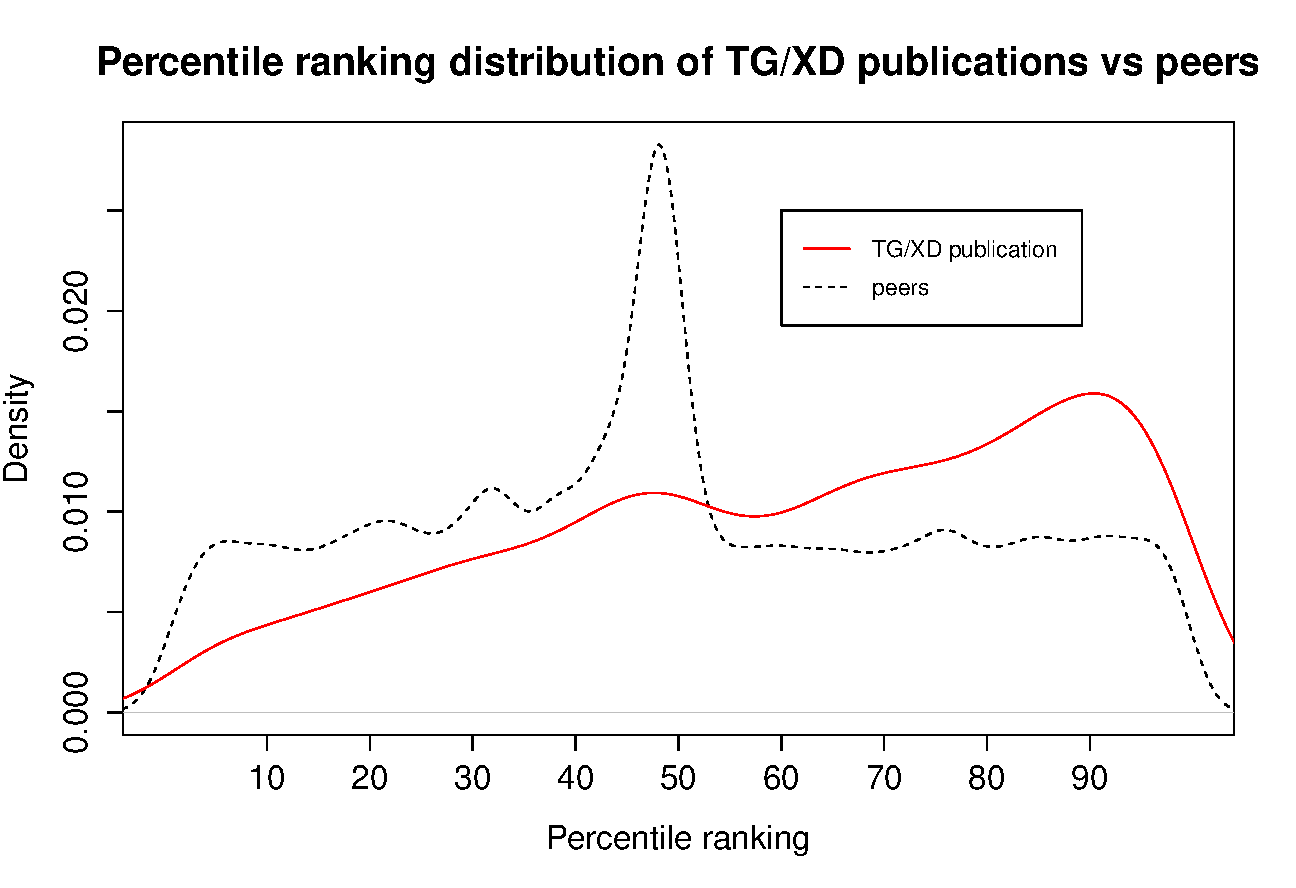
\includegraphics[width=1.0\columnwidth]{images-new/xd_peers_density.pdf} 
  \caption{Kernel density of distributions for XSEDE publication percentile ranking versus peers.}\label{F:xd_peers_density} 

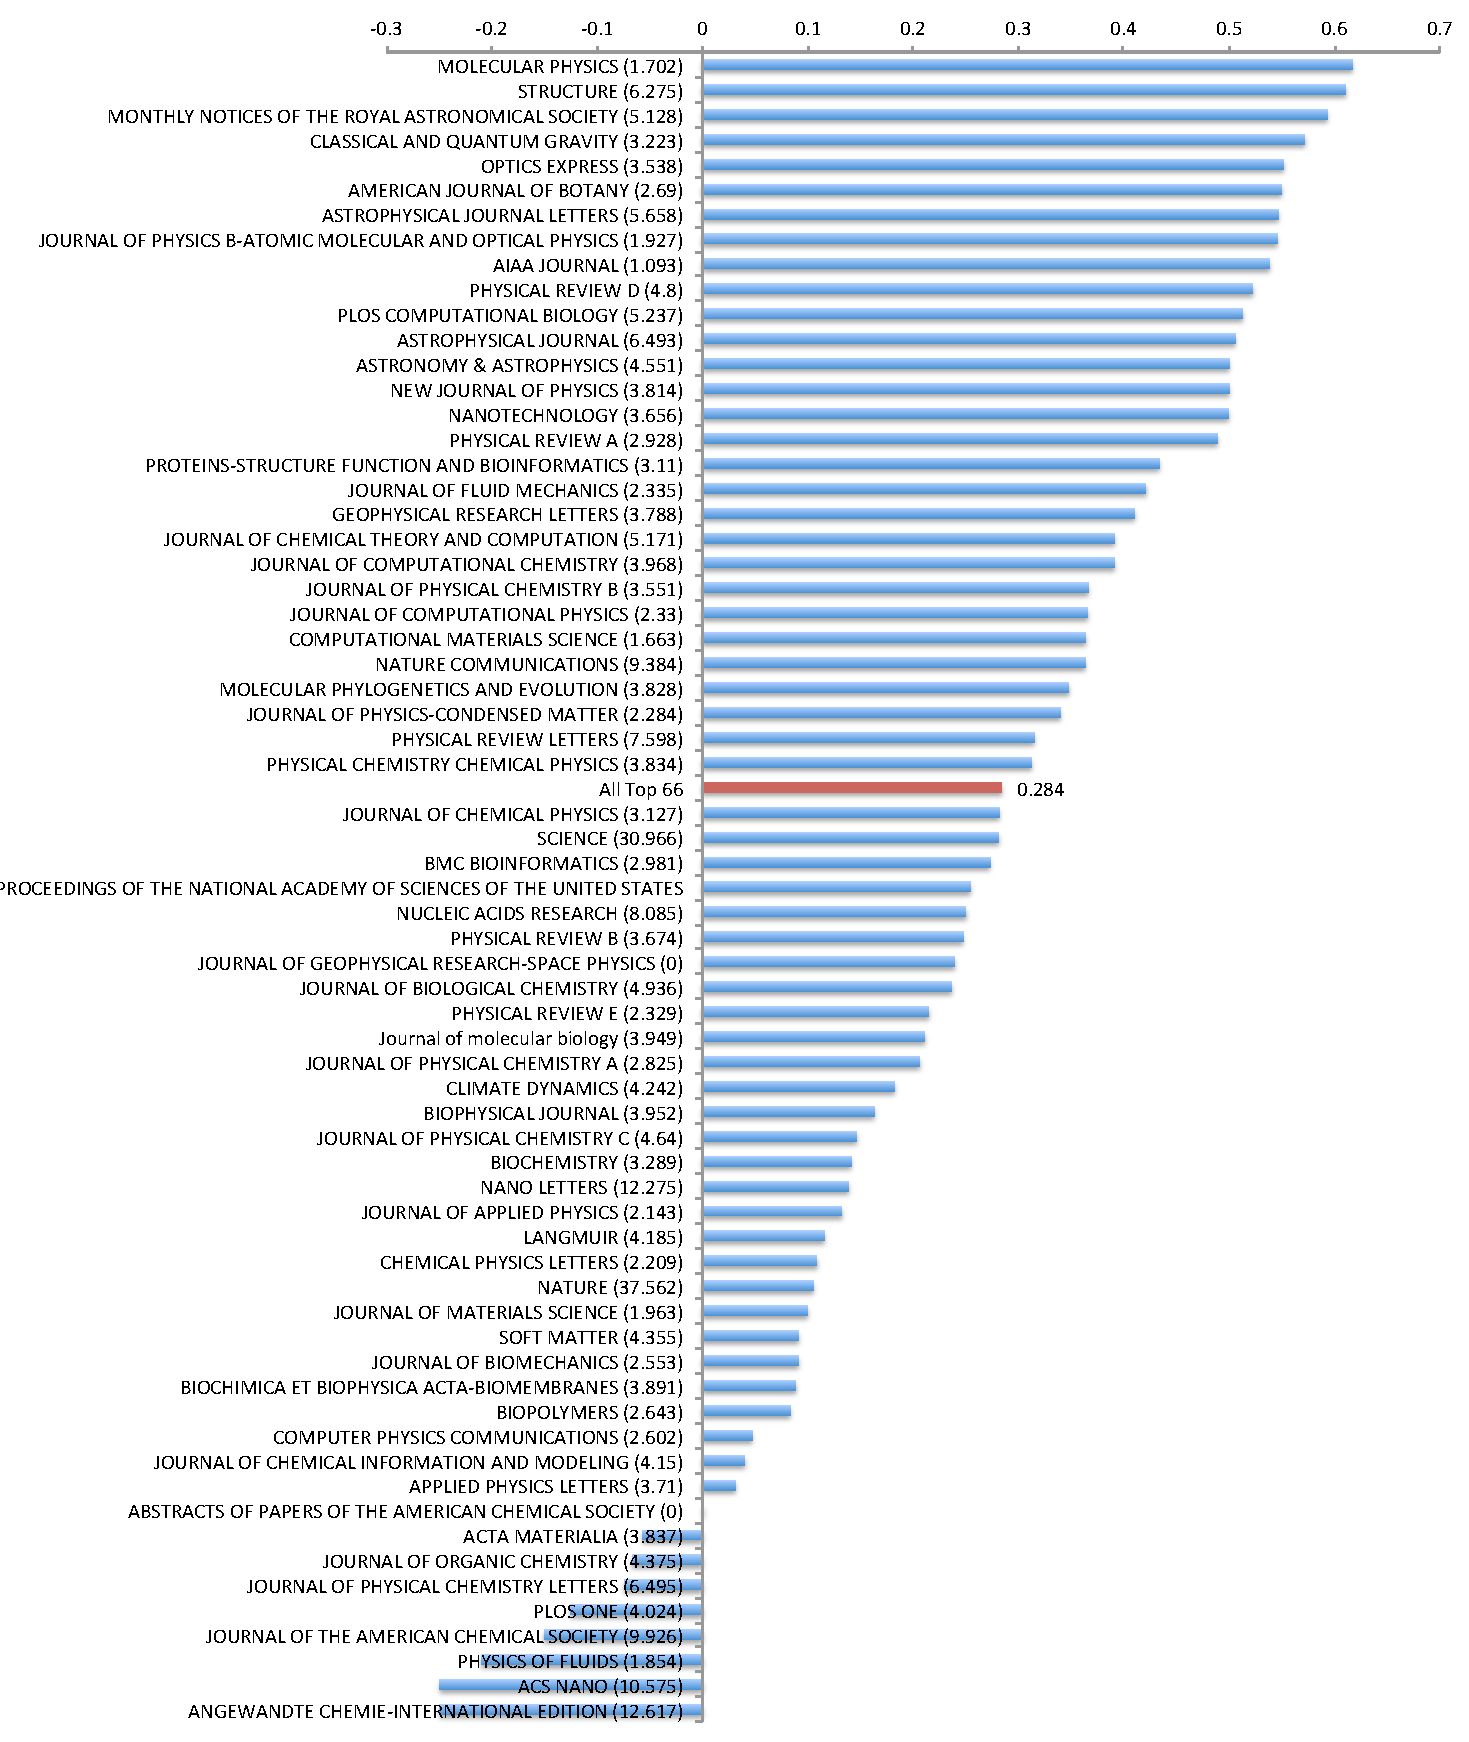
\includegraphics[width=.9\columnwidth]{images-new/xsede-journal-score.pdf} 
\caption{The score of our peer comparison metric for XSEDE publications by journal.}\label{F:xsede-score} 
    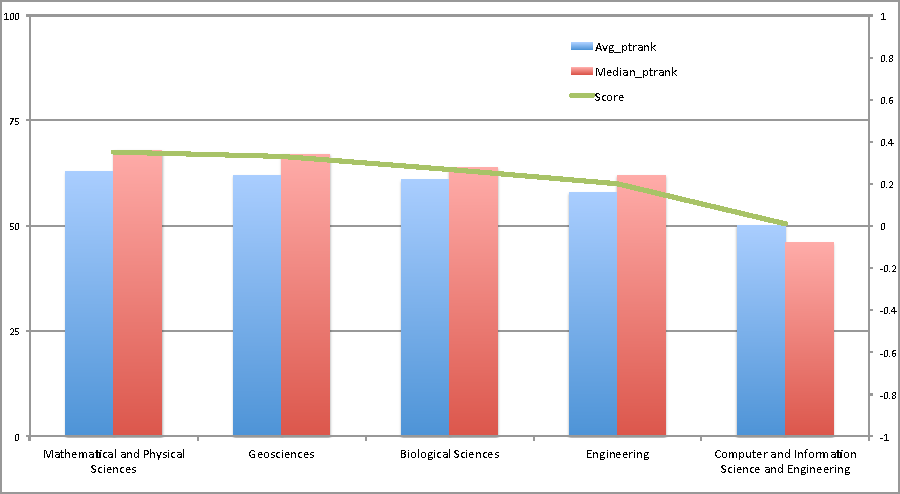
\includegraphics[width=1.0\columnwidth]{images-new/c.pdf} 
  \caption{Peers comparison based on the topmost Field of Science category as defined by NSF.}\label{F:xsede-top-c} 

\hfill

\end{figure} 

\begin{table}[h!]
\caption{Basic statistics of XSEDE publications group and peers group}
\label{T:groups_stats}
\centering
\begin{small}
\begin{tabular}{lrrrrrr}
 & Number of & \multicolumn{2}{ c }{Rank} & \multicolumn{2}{ c }{Citations}  \\
 &  Publications & Average & Median & Average & Median \\
\hline
  XD     & 2349	        & 61	& 65	& 26	& 11 \\
Peers & 168422	& 49	& 48	& 13	& 5 \\
\end{tabular}
\end{small}
\end{table}


\begin{figure*}[htb!] 
  \centering 
    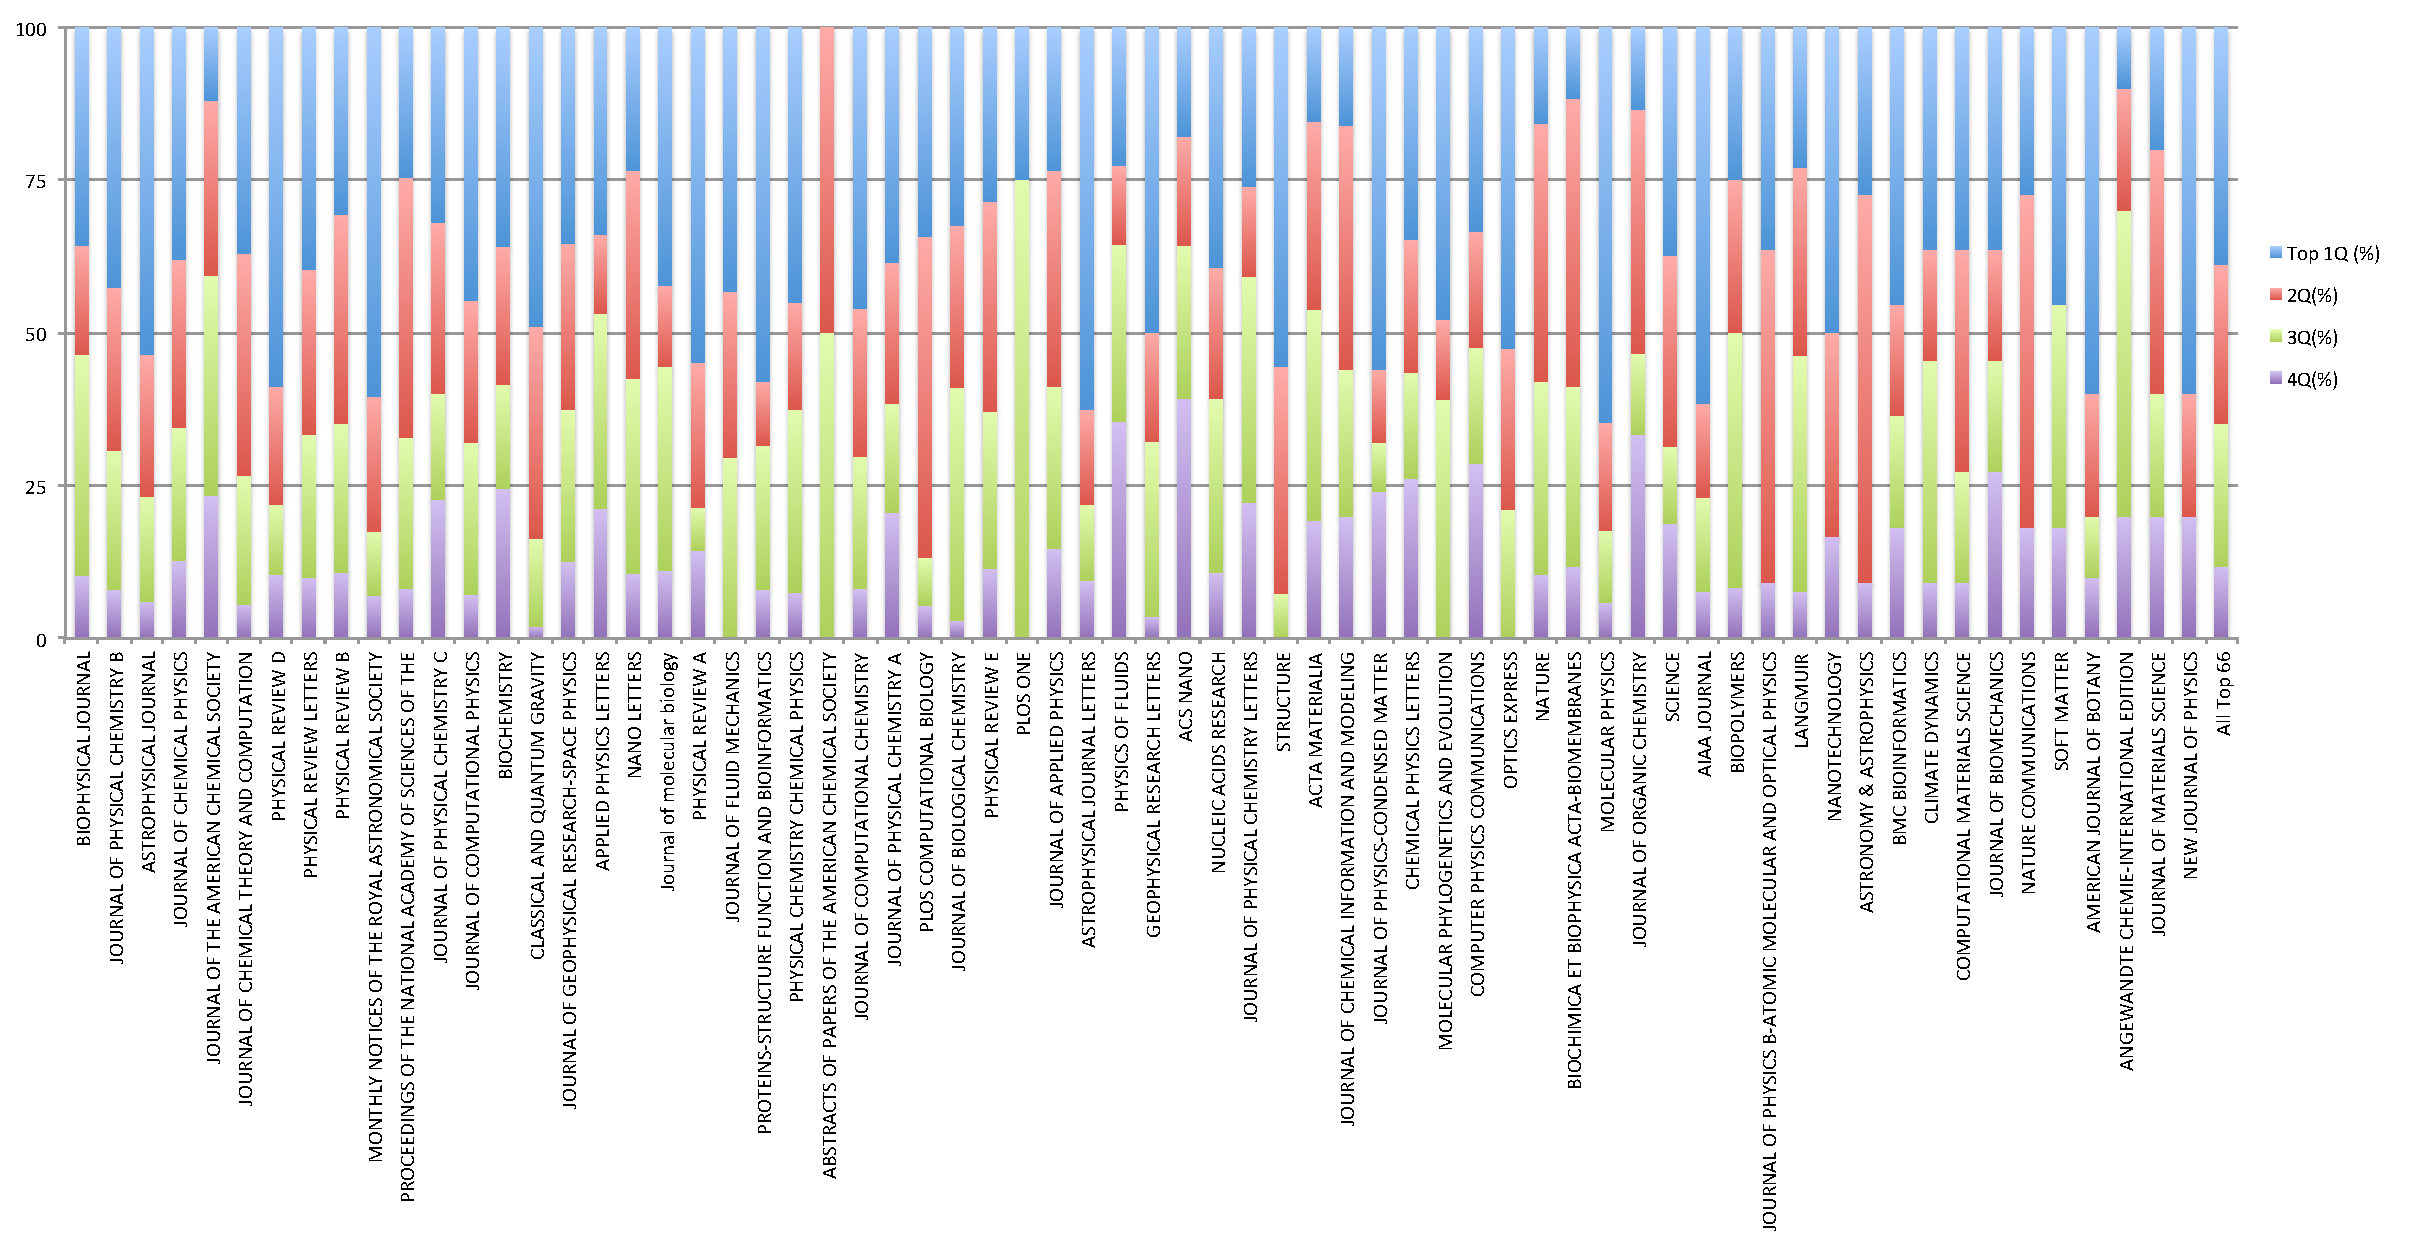
\includegraphics[width=1.0\textwidth]{images-new/xsede-journal-stacked.pdf} 
  \caption{Percentile ranging by FOS in a stacked barchart of XSEDE publications.}\label{F:xsede-stacked} 
\end{figure*}

\bigskip

\begin{figure*}[htb!] 
  \centering 
    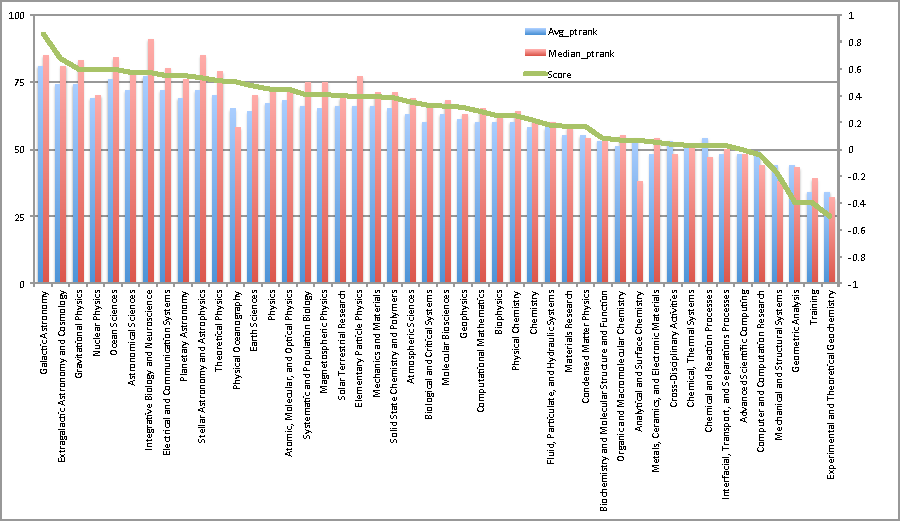
\includegraphics[width=.9\textwidth]{images-new/a.pdf} 
  \caption{Peer comparison based on Field of Science of XSEDE publications.}\label{F:xsede-fos-a} 

  \centering 
    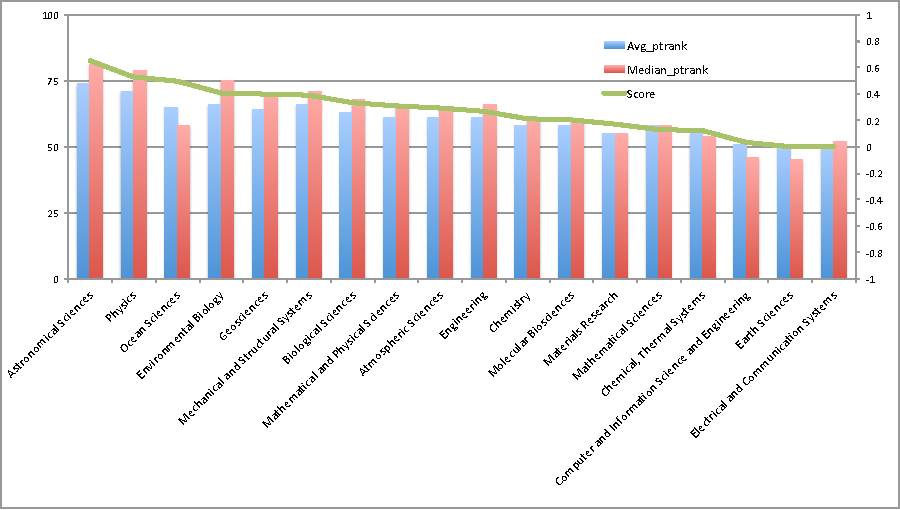
\includegraphics[width=.9\textwidth]{images-new/b.pdf} 
  \caption{Peer comparison based on Parent Field of Science from the original analysis of XSEDE data.}\label{F:xsede-stacked-b} 

\end{figure*} 

The results are depicted in Figures \ref{F:xsede-stacked}, \ref{F:xsede-fos-a}, \ref{F:xsede-stacked-b}, \ref{F:xsede-score}, and \ref{F:xsede-top-c}. 

NSF and XSEDE define a hierarchy of FOSs. In Figure \ref{F:xsede-top-c}, we show the top level FOS as defined by NSF. When we look to expand the FOS to the next level in the hierarchy, we find the results as depicted in Figure \ref{F:xsede-stacked-b}. The next level is shown in Figure \ref{F:xsede-fos-a}. Each of these figures shows the list of FOSs in decreasing order by the performance score $S$. 

From Figure \ref{F:xsede-fos-a} we can identify that for most fields of science the XSEDE publications performed better than their peers. The average and median scores were higher than 50 and the score is positive. When looking at individual results, we see that astronomy and physics benefit most from using XSEDE/TG. When looking at the fields that perform worst, we find fields such as Experimental and Theoretical Geochemistry, Geometric Analysis and Mechanical and Structural systems. Such fields are typically not dominated by simulation science and are less dependent on computational resources. Other fields such as Training include many other areas of training outside of supercomputing usage. We even find fields such as Computer and Computation Research to be less impacted. We certainly have to acknowledge in this case that many theoretical papers and papers not using supercomputers are published. 

To show the percentile distribution in more detail for each journal, we present in Figure \ref{F:xsede-stacked} a stacked barchart. Also here, as expected from our previous results, we see a positive impact in the percentile citation count for most of the journals. This is made obvious by looking at Figure \ref{F:xsede-score}. Here we also have included the average of the top 66 journals in which we found 10 or more XSEDE publications and find that the score metric is positive with a value of 0.284. Thus we can conclude that papers benefit from use of XSEDE resources, based on self-identification in reports and bibliographic upload to the XSEDE portal, resulting in their being more cited on average than their peers from the same journal.

\section{NCAR Peer Data Analysis}\label{S:ncar}

\begin{figure}[h!] 
  \centering 
    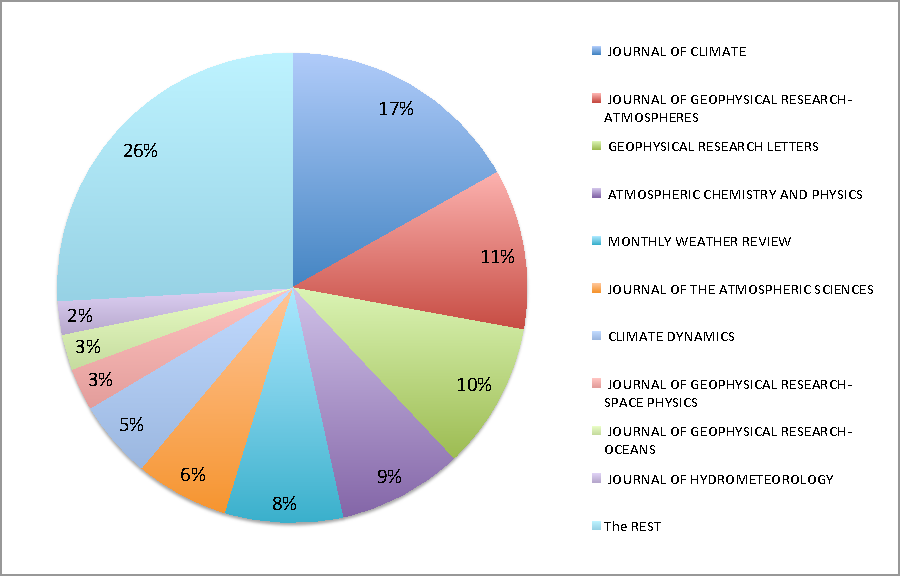
\includegraphics[width=0.75\columnwidth]{images-new/ncar-a.pdf} 
  \caption{Distribution of the top most journals by publication count.}\label{F:ncar-distribution} 

  \centering 
    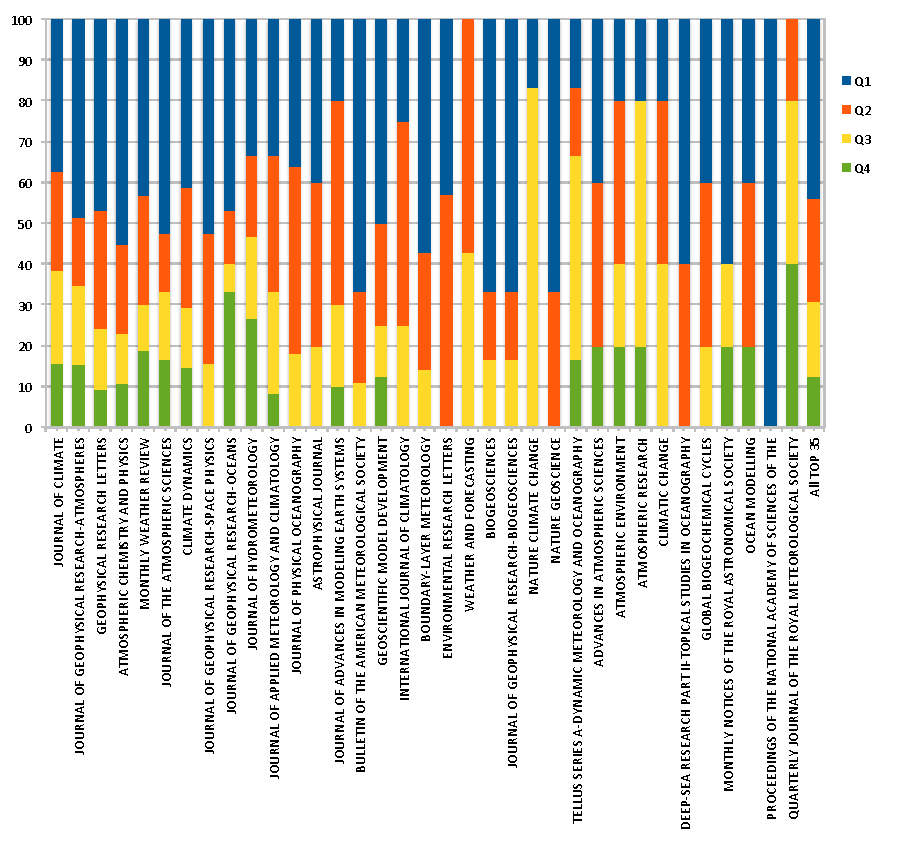
\includegraphics[width=1.0\columnwidth]{images-new/ncar-b.pdf} 
  \caption{Percentile ranging by FOS in a stacked barchart of NCAR publications.}\label{F:ncar-stacked-b} 

  \centering 
    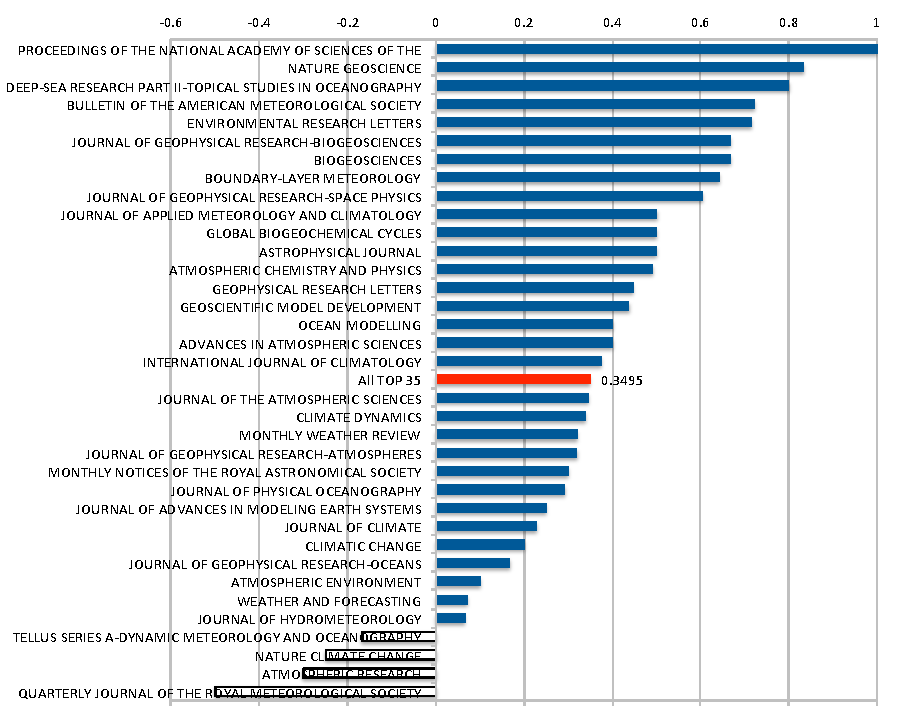
\includegraphics[width=1.0\columnwidth]{images-new/ncar-c.pdf} 
  \caption{Peer comparison based on Parent Field of Science from the original analysis of XSEDE data.}\label{F:ncar-score}
\end{figure} 

We have replicated the publication citation analysis with a text file of 880 publications obtained from NCAR. Because the NCAR data set was smaller than the one from XSEDE, instead of looking at all journals that have at least ten publications, we reduced the value to five. This will give a large enough journal number to conduct our analysis in this case. To conduct the analysis, we took the following steps.

\begin{enumerate}

\item We parsed the text file containing 880 publications into a structured database while identifying titles, and DOIs.

\item With our framework, we queried ISI Web of Knowledge to get detailed information on the publications -- journal name, issue, citation data and other identifying information. We were able to verify and obtain data for 813 publications.

\item Through our framework, we identified and obtained peer data based on journal issue information. In total, 130 different publication venues have been identified. To ensure the results are statistically meaningful, we eliminated those with less than five publications appearing in them.  This leads to 35 different journals that cover 653 publications. Out of the 35 journals, we had peers data for 12 of them (from our XSEDE peers comparison work). For the other 23 journals, we obtained peer publication data for an additional 39,000 publications.

\item For each NCAR publication, we computed the percentile ranking among peers within the same journal issue against all publication entries as obtained from ISI Web of Knowledge.

\item We grouped the percentile ranking scores based on each journal, divided the scores into each ranking quarters ($Q_1$: top 25\%; top $Q_2$: 25\%~50\%; bottom $Q_3$: 50\%-75\%, bottom $Q_4$: 75\%-100\%), and computed the percentage for those that fall into each ranking quarter.

\end{enumerate}

We depict the result in a stacked column chart similar to that used in Figure \ref{F:xsede-stacked}.  In Figure \ref{F:ncar-distribution}, we show the distribution of the publications in the top 10 journals sorted by the number of publications. The top 10 journals total 484 publications. They account for about three quarters of the 653 publications from the 35 journals with at least five publications appearing in them; or 60\% of the 813 publications from the 130 journals we identified via the ISI source (see Table~\ref{T:ncar-pub-count-venue}).

We also computed and compared the \emph{performance score} as defined earlier. The result is shown in Figure \ref{F:ncar-score}. Here we see that the average over all 35 entries is a positive value of about 0.35. 

\section{Conclusion} \label{S:conclusion}

We observe that the NCAR score is slightly higher than that of XSEDE. However, we need to take into account that XSEDE publications have a wider range of FOS; NCAR focusses on a much narrower FOS. Furthermore, as we can see from the XSEDE results, research in the atmospheric sciences resulted in the highest score values using XSEDE resources. Thus we can understand that the value is higher for NCAR as they do not include the other disciplines that have lower values.

However, the most important conclusion we make for our metric is that, for both XSEDE and NCAR publications, the impact measured by a percentile score is positive and higher than their peers that have not used such resources. 

We will further expand upon our metric and can define such values also for other groups defined in XSEDE or for other resource providers. The important information we need is a reliable source that identifies publications that can be associated with the resource. While exploring not only XSEDE, but also NCAR data we have in principle shown that our approach is applicable to other resource providers.

%%%%%%%%%%%%%%%%%%%%%%%%%%%%%%%%%%%%%%%%%%%%%%%%%%%%%%%%%%%%%%%%%%%%%% 
% Acknowledgment 
%%%%%%%%%%%%%%%%%%%%%%%%%%%%%%%%%%%%%%%%%%%%%%%%%%%%%%%%%%%%%%%%%%%%%% 

\section{Acknowledgments}

 
This work is part of the Technology Auditing Service (TAS) project sponsored by NSF under grant number OCI-1025159. Lessons learned from FutureGrid have significantly influenced this work. Gathering publications was first pioneered by FutureGrid, influencing the development in the XSEDE portal. We would like to thank Matt Hanlon and Maytal Dahan for their efforts to integrate this framework into the XSEDE portal. 
 
%\bibliographystyle{IEEEtranS}
%\bibliographystyle{IEEEtran}
\bibliographystyle{abbrvurl} 
\bibliography{% 
bib/tas,%
bib/vonlaszewski-new} 

\end{document}

%%%%%%%%%%%%%%%%%%%%%%%%%%%%%%%%%%%%%%%%%%%%%%%%%%%%%%%%%%%%%%%%%%%%%%
%%%%%%%%%%%%%%%%%%%%%%%%%%%%%%%%%%%%%%%%%%%%%%%%%%%%%%%%%%%%%%%%%%%%%%
%%%%%%%%%%%%%%%%%%%%%%%%%%%%%%%%%%%%%%%%%%%%%%%%%%%%%%%%%%%%%%%%%%%%%%

% END END 

%%%%%%%%%%%%%%%%%%%%%%%%%%%%%%%%%%%%%%%%%%%%%%%%%%%%%%%%%%%%%%%%%%%%%%
%%%%%%%%%%%%%%%%%%%%%%%%%%%%%%%%%%%%%%%%%%%%%%%%%%%%%%%%%%%%%%%%%%%%%%
%%%%%%%%%%%%%%%%%%%%%%%%%%%%%%%%%%%%%%%%%%%%%%%%%%%%%%%%%%%%%%%%%%%%%%